\documentclass[14pt]{extbook}
\usepackage{multicol, enumerate, enumitem, hyperref, color, soul, setspace, parskip, fancyhdr} %General Packages
\usepackage{amssymb, amsthm, amsmath, bbm, latexsym, units, mathtools} %Math Packages
\everymath{\displaystyle} %All math in Display Style
% Packages with additional options
\usepackage[headsep=0.5cm,headheight=12pt, left=1 in,right= 1 in,top= 1 in,bottom= 1 in]{geometry}
\usepackage[usenames,dvipsnames]{xcolor}
\usepackage{dashrule}  % Package to use the command below to create lines between items
\newcommand{\litem}[1]{\item#1\hspace*{-1cm}\rule{\textwidth}{0.4pt}}
\pagestyle{fancy}
\lhead{Progress Quiz 5}
\chead{}
\rhead{Version C}
\lfoot{9912-2038}
\cfoot{}
\rfoot{Spring 2021}
\begin{document}

\begin{enumerate}
\litem{
Determine the vertical asymptotes and holes in the rational function below.\[ f(x) = \frac{12x^{3} -35 x^{2} +7 x + 30}{9x^{2} -3 x -20} \]\begin{enumerate}[label=\Alph*.]
\item \( \text{Vertical Asymptotes of } x = -1.333 \text{ and } x = -0.75 \text{ with a hole at } x = 1.667 \)
\item \( \text{Vertical Asymptote of } x = 1.333 \text{ and hole at } x = 1.667 \)
\item \( \text{Holes at } x = -1.333 \text{ and } x = 1.667 \text{ with no vertical asymptotes.} \)
\item \( \text{Vertical Asymptotes of } x = -1.333 \text{ and } x = 1.667 \text{ with no holes.} \)
\item \( \text{Vertical Asymptote of } x = -1.333 \text{ and hole at } x = 1.667 \)

\end{enumerate} }
\litem{
Determine the vertical asymptotes and holes in the rational function below.\[ f(x) = \frac{8x^{3} -26 x^{2} -5 x + 50}{16x^{2} +32 x + 15} \]\begin{enumerate}[label=\Alph*.]
\item \( \text{Vertical Asymptote of } x = 0.5 \text{ and hole at } x = -1.25 \)
\item \( \text{Vertical Asymptotes of } x = -0.75 \text{ and } x = 2.5 \text{ with a hole at } x = -1.25 \)
\item \( \text{Holes at } x = -0.75 \text{ and } x = -1.25 \text{ with no vertical asymptotes.} \)
\item \( \text{Vertical Asymptotes of } x = -0.75 \text{ and } x = -1.25 \text{ with no holes.} \)
\item \( \text{Vertical Asymptote of } x = -0.75 \text{ and hole at } x = -1.25 \)

\end{enumerate} }
\litem{
Determine the horizontal and/or oblique asymptotes in the rational function below.\[ f(x) = \frac{16x^{3} +48 x^{2} +47 x + 15}{8x^{3} +24 x^{2} +27 x + 9} \]\begin{enumerate}[label=\Alph*.]
\item \( \text{None of the above} \)
\item \( \text{Horizontal Asymptote of } y = 0  \)
\item \( \text{Vertical Asymptote of } y = -1.500  \)
\item \( \text{Vertical Asymptote of } y = -1  \)
\item \( \text{Horizontal Asymptote of } y = 2.000  \)

\end{enumerate} }
\litem{
Determine the vertical asymptotes and holes in the rational function below.\[ f(x) = \frac{6x^{3} +37 x^{2} +67 x + 30}{6x^{2} +13 x + 6} \]\begin{enumerate}[label=\Alph*.]
\item \( \text{Holes at } x = -1.5 \text{ and } x = -0.667 \text{ with no vertical asymptotes.} \)
\item \( \text{Vertical Asymptotes of } x = -1.5 \text{ and } x = -0.667 \text{ with no holes.} \)
\item \( \text{Vertical Asymptote of } x = -1.5 \text{ and hole at } x = -0.667 \)
\item \( \text{Vertical Asymptotes of } x = -1.5 \text{ and } x = -2.5 \text{ with a hole at } x = -0.667 \)
\item \( \text{Vertical Asymptote of } x = 1.0 \text{ and hole at } x = -0.667 \)

\end{enumerate} }
\litem{
Determine the vertical asymptotes and holes in the rational function below.\[ f(x) = \frac{9x^{3} -27 x^{2} -16 x + 48}{9x^{2} -3 x -20} \]\begin{enumerate}[label=\Alph*.]
\item \( \text{Vertical Asymptotes of } x = 1.667 \text{ and } x = -1.333 \text{ with no holes.} \)
\item \( \text{Holes at } x = 1.667 \text{ and } x = -1.333 \text{ with no vertical asymptotes.} \)
\item \( \text{Vertical Asymptote of } x = 1.0 \text{ and hole at } x = -1.333 \)
\item \( \text{Vertical Asymptote of } x = 1.667 \text{ and hole at } x = -1.333 \)
\item \( \text{Vertical Asymptotes of } x = 1.667 \text{ and } x = 1.333 \text{ with a hole at } x = -1.333 \)

\end{enumerate} }
\litem{
Which of the following functions \textit{could} be the graph below?
\begin{center}
    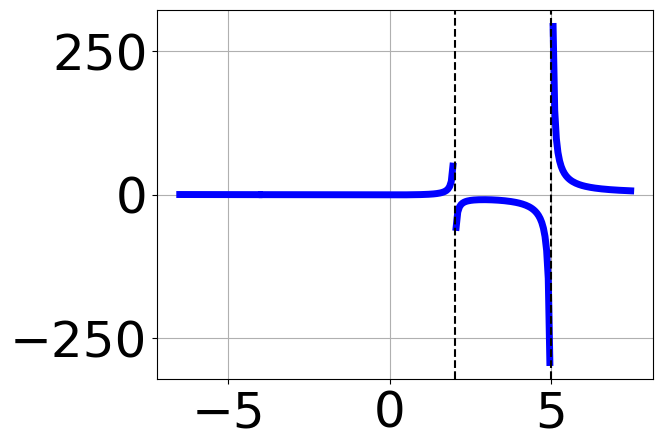
\includegraphics[width=0.5\textwidth]{../Figures/identifyGraphOfRationalFunctionCopyC.png}
\end{center}
\begin{enumerate}[label=\Alph*.]
\item \( f(x)=\frac{x^{3} +9 x^{2} +14 x -24}{x^{3} -3 x^{2} -18 x + 40} \)
\item \( f(x)=\frac{x^{3} +10 x^{2} +19 x -30}{x^{3} -3 x^{2} -18 x + 40} \)
\item \( f(x)=\frac{x^{3} -9 x^{2} +14 x + 24}{x^{3} +3 x^{2} -18 x -40} \)
\item \( f(x)=\frac{x^{3} -9 x^{2} +14 x + 24}{x^{3} +3 x^{2} -18 x -40} \)
\item \( \text{None of the above are possible equations for the graph.} \)

\end{enumerate} }
\litem{
Determine the horizontal and/or oblique asymptotes in the rational function below.\[ f(x) = \frac{6x^{3} -1 x^{2} -75 x + 100}{3x^{2} +7 x -20} \]\begin{enumerate}[label=\Alph*.]
\item \( \text{Horizontal Asymptote at } y = -4.0 \)
\item \( \text{Oblique Asymptote of } y = 2x -5. \)
\item \( \text{Horizontal Asymptote of } y = -4.0 \text{ and Oblique Asymptote of } y = 2x -5 \)
\item \( \text{Horizontal Asymptote of } y = 2.0 \text{ and Oblique Asymptote of } y = 2x -5 \)
\item \( \text{Horizontal Asymptote of } y = 2.0  \)

\end{enumerate} }
\litem{
Determine the horizontal and/or oblique asymptotes in the rational function below.\[ f(x) = \frac{8x^{3} +54 x^{2} +103 x + 60}{4x^{3} -6 x^{2} -64 x -80} \]\begin{enumerate}[label=\Alph*.]
\item \( \text{None of the above} \)
\item \( \text{Vertical Asymptote of } y = 4.000  \)
\item \( \text{Vertical Asymptote of } y = -4  \)
\item \( \text{Horizontal Asymptote of } y = 2.000  \)
\item \( \text{Horizontal Asymptote of } y = 0  \)

\end{enumerate} }
\litem{
Determine the horizontal and/or oblique asymptotes in the rational function below.\[ f(x) = \frac{8x^{3} -38 x^{2} +55 x -25}{4x^{2} +3 x -10} \]\begin{enumerate}[label=\Alph*.]
\item \( \text{Horizontal Asymptote of } y = 2.0 \text{ and Oblique Asymptote of } y = 2x -11 \)
\item \( \text{Oblique Asymptote of } y = 2x -11. \)
\item \( \text{Horizontal Asymptote at } y = -2.0 \)
\item \( \text{Horizontal Asymptote of } y = -2.0 \text{ and Oblique Asymptote of } y = 2x -11 \)
\item \( \text{Horizontal Asymptote of } y = 2.0  \)

\end{enumerate} }
\litem{
Which of the following functions \textit{could} be the graph below?
\begin{center}
    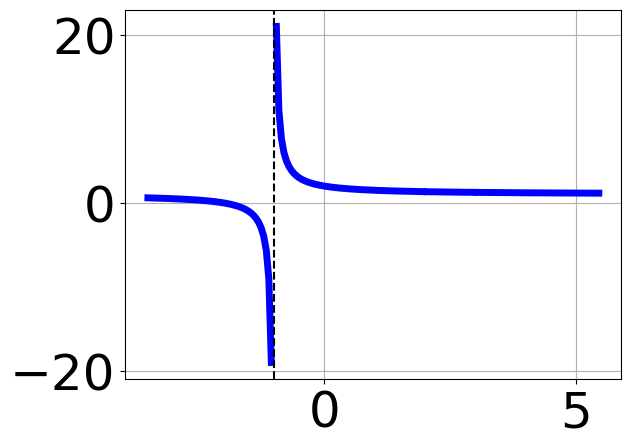
\includegraphics[width=0.5\textwidth]{../Figures/identifyGraphOfRationalFunctionC.png}
\end{center}
\begin{enumerate}[label=\Alph*.]
\item \( f(x)=\frac{x^{3} +3 x^{2} -4 x -12}{x^{3} +4 x^{2} +x -6} \)
\item \( f(x)=\frac{x^{3} +6 x^{2} +3 x -10}{x^{3} -4 x^{2} +x + 6} \)
\item \( f(x)=\frac{x^{3} -3 x^{2} -4 x + 12}{x^{3} -4 x^{2} +x + 6} \)
\item \( f(x)=\frac{x^{3} +3 x^{2} -4 x -12}{x^{3} +4 x^{2} +x -6} \)
\item \( \text{None of the above are possible equations for the graph.} \)

\end{enumerate} }
\end{enumerate}

\end{document}